\documentclass[conference]{IEEEtran}
\IEEEoverridecommandlockouts
% The preceding line is only needed to identify funding in the first footnote. If that is unneeded, please comment it out.
\usepackage[utf8]{inputenc} % allow utf-8 input
\usepackage[T1]{fontenc}    % use 8-bit T1 fonts
\usepackage{hyperref}       % hyperlinks
\usepackage{url}            % simple URL typesetting
\usepackage{booktabs}       % professional-quality tables
\usepackage{nicefrac}       % compact symbols for 1/2, etc.
\usepackage{microtype}      % microtypography
\usepackage{multicol}
\usepackage{multirow}
\usepackage{diagbox}
\usepackage{subfigure}
\usepackage{tabularx}
\usepackage{cite}
\usepackage{amsmath,amssymb,amsfonts}
\usepackage{algorithmic}
\usepackage{graphicx}
\usepackage{textcomp}
\usepackage{xcolor}
\usepackage{indentfirst}
\def\BibTeX{{\rm B\kern-.05em{\sc i\kern-.025em b}\kern-.08em
    T\kern-.1667em\lower.7ex\hbox{E}\kern-.125emX}}
\begin{document}
\bibliographystyle{IEEEtran}

\title{Principles of Data Science Project 3\\
Feature Encoding}

\author{\IEEEauthorblockN{Hongzhou Liu}
\IEEEauthorblockA{517030910214}
\texttt{deanlhz@sjtu.edu.cn}
\and
\IEEEauthorblockN{Xuanrui Hong}
\IEEEauthorblockA{517030910227}
\texttt{hongxuanrui.1999@sjtu.edu.cn}
\and
\IEEEauthorblockN{Qilin Chen}
\IEEEauthorblockA{517030910155}
\texttt{1017856853@sjtu.edu.cn}
}

\maketitle

\begin{abstract}
Hello
\end{abstract}

\begin{IEEEkeywords}
something
\end{IEEEkeywords}

\section{Introduction}
\subsection{SIFT}
Scale-invariant feature transform (SIFT) is a machine vision algorithm used to detect and describe local features in an image. It looks for extreme points in the spatial scale and extracts its position, scale, rotation invariant. This algorithm was published by David Lowe in 1999, and was summarized in 2004.\cite{lowe1999object} The description and detection of local image features can help identify objects. SIFT features are based on some local appearance points of interest on the object and are not related to the size and rotation of the image. The tolerance to light, noise, and slight changes in viewing angle is also quite high. Based on these characteristics, they are highly conspicuous and relatively easy to capture. In a huge feature database, objects are easy to identify and rarely misidentified.\par
The main steps of the sift algorithm are as follows:
\subsubsection{Scale-space extrema detection}The images are convolved with Gaussian filters at different scales, and then continuous Gaussian blur is used to blur the image differences to find the key points. The key point is based on the maximum and minimum Gaussian difference (DoG) at different scales. In other words, the $D(x,y,\sigma)$ of the DoG image is caused by:\begin{equation}
D(x,y,\sigma)=L(x,y,k_i\sigma)-L(x,y,k_j\sigma)
\end{equation}
\begin{center}
	\begin{figure}[htbp]
		\centering
		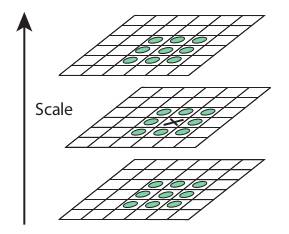
\includegraphics[width=5cm]{image/sift_local_extrema.jpg}
		\caption{Local Extrema}
	\end{figure}
\end{center}
$L(x,y,k\sigma)$ is the convolution of the original image $I(x,y)$ and Gaussian blur $G(x,y,k\sigma)$ under the condition of the scale $k\sigma$, for example:
\begin{equation}
L(x,y,\sigma)=G(x,y,k\sigma)\times I(x,y)
\end{equation}
$G(x,y,k\sigma)$ is a variable-scale Gaussian function:
\begin{equation}
G(x,y,\sigma) = \frac{1}{2\Pi\sigma^2}e^{-(x^2+y^2)/2\sigma^2}
\end{equation}\par
Once the DoG image is obtained, the maximum and minimum values in the DoG image can be found as key points. In order to determine the key points, each pixel in the DoG image will be made with eight pixels around the center of itself, and nine pixels in the same position of the adjacent scale magnification in the same group of DoG images, for a total of 26 points. For comparison, if this pixel is the maximum and minimum of these twenty-six pixels, this pixel is called a key point.
\begin{center}
	\begin{figure}[htbp]
		\centering
		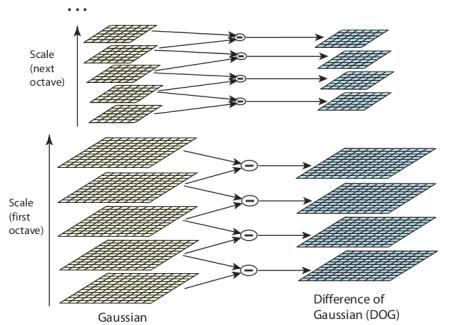
\includegraphics[width=5cm]{image/sift_dog.jpg}
		\caption{DoG}
	\end{figure}
\end{center}
\subsubsection{Keypoint localization}
There may be too many key points in different size spaces, and some key points may be relatively difficult to identify or susceptible to noise interference. The next step of the SIFT algorithm will locate each key point by the information of pixels near the key point, the size of the key point, and the main curvature of the key point, thereby eliminating the key points that are located on the side or are susceptible to noise
\subsubsection{Orientation assignment}
After the above steps, feature points that exist at different scales have been found. In order to achieve image rotation invariance, the direction of the feature points needs to be assigned. Use the gradient distribution characteristics of the pixels in the neighborhood of the feature point to determine its direction parameters, and then use the gradient histogram of the image to find the stable direction of the local structure of the key point.
\subsubsection{Keypoint descriptor}
Through the above steps, the location, scale and direction information of SIFT feature points have been found. Next, use a set of vectors to describe the key points, that is, to generate feature point descriptors. There are roughly three steps in generating feature descriptors:
\begin{itemize}
\item Correct the main direction of rotation to ensure rotation invariance.
\item Generate descriptors and ultimately form a 128-dimensional feature vector
\item In the normalization process, the feature vector length is normalized to further remove the influence of lighting.
\end{itemize}

\subsection{Selective Search}

Selective Search is a object recognition algorithm which combines the strength of both an exhaustive search and segmentation.\cite{2013Selective} We know that the problem of target detection is more complicated than image classification. An important reason is that there may be multiple objects in an image that need to be located and classified separately. Obviously, before training the classifier, you need to use some methods to divide the image into small areas. Selective search method has three main advantages: capture different scales, diversification, fast to compute. Selective search algorithm mainly includes two steps: hierarchical grouping algorithm and diversification strategies, which can be summed as follows:

\subsubsection{Hierarchical Grouping Algorithm}

Hierarchical grouping algorithm use the method of Felzenszwalb and Huttenlocher to generate the initial region of the image, and use the greedy algorithm to iteratively group the regions. In each grouping iteration, a larger area is formed and added to the area proposal list. Algorithm will create a regional proposal from smaller segments to larger segments in a bottom-up behavior, as shown in Fig. \ref{kFig1}.
\begin{center}
	\begin{figure}
		\centering
		\subfigure{
			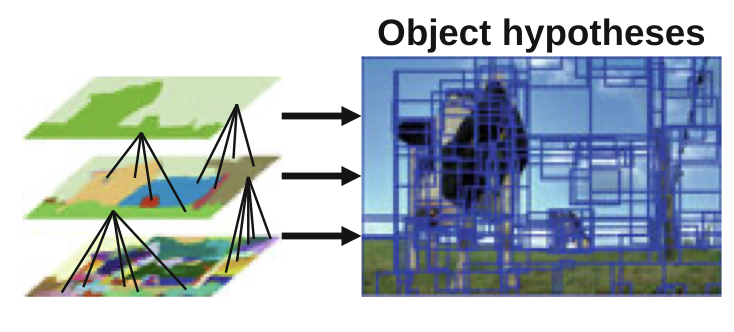
\includegraphics[width=8cm]{image/level.jpg}
		}
		\caption{Hierarchical Grouping Algorithm.\cite{2013Selective}}
		\label{kFig1}
	\end{figure}
\end{center}
\subsubsection{Diversification Strategies}
In order to diversify the sampling in grouping, selective search algorithm present three diversification strategies:
\begin{itemize}
\item Use various color spaces.
\item Use different similarity measures.
\item Changing the starting area to make sampling.
\end{itemize}


\subsection{ResNet}
Residual Network (ResNet) \cite{He2016Deep} is presented to ease the training of networks that are substantially deeper than those used previously and have the best performance in ILSVRC \& COCO 2015 competitions. We can conclude its motivation that ResNet add a skip connection in every building blocks to solve the degradation problem as the learning networks become deeper and deeper. The framework of ResNet can be show in Fig. \ref{kFig0}. We can express its principle by the following expression:
$$x_{i}=x_{i-1}+F(x_{i-1})$$
where $x_{i}$ is the network input and $x_{i-1}$ is the output, $F(\cdot)$ present the transform of network block.

As an state-of-the-art model in deeplearning feild, its skip connection structure can be seen as a smoother in training process \cite{Veit2016Residual}, and the information can be maintained in forword training, which can be seen in the network loss \cite{touretzky1996advances}.

\begin{center}
	\begin{figure}
		\centering
		\subfigure{
			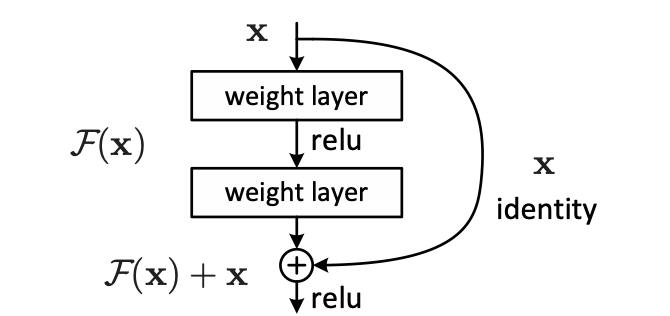
\includegraphics[width=8cm]{image/resnet.jpg}
		}
		\caption{Residual learning: a building block.\cite{He2016Deep}}
		\label{kFig0}
	\end{figure}
\end{center}

\section{Experiments}
\subsection{Sift descriptors}
We used sift to extract the local descriptors of the images, and then used BOW, VLAD, FV to encode the features, and finally put them into the SVM for classification. As shown in fig. \ref{Fig1}, when using sift to extract local descriptors, we encountered some images that could not be extracted. We improved the image contrast to processe these images, and finally got the results.
\begin{center}
	\begin{figure}
		\centering
		\subfigure[original image]{
			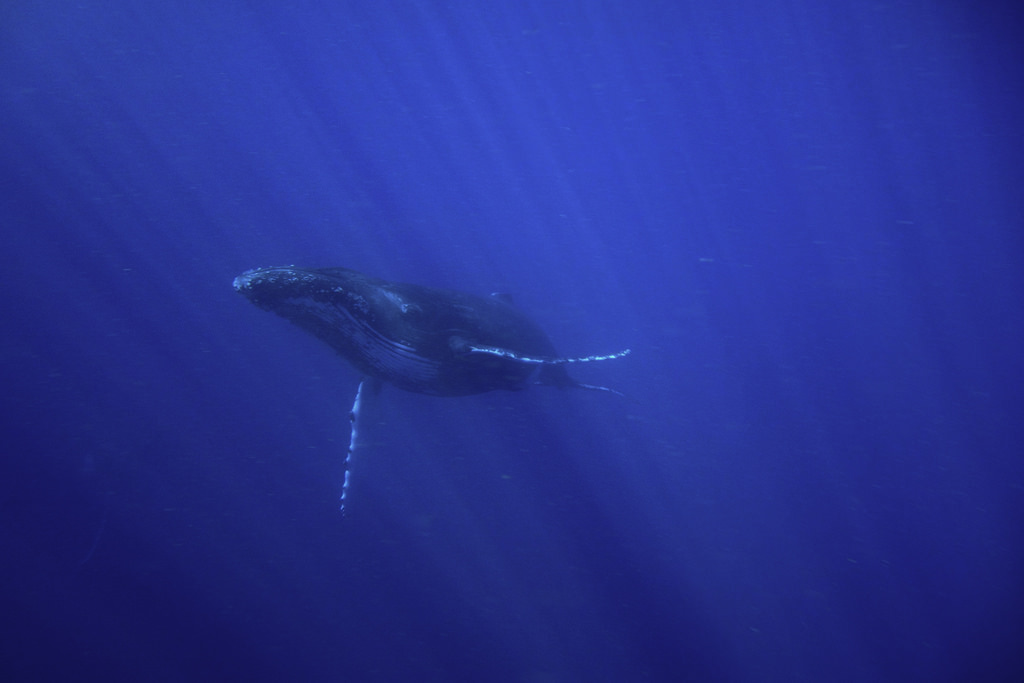
\includegraphics[width=5cm]{image/origin.jpg}
		}
		\quad
		\subfigure[processed image]{
			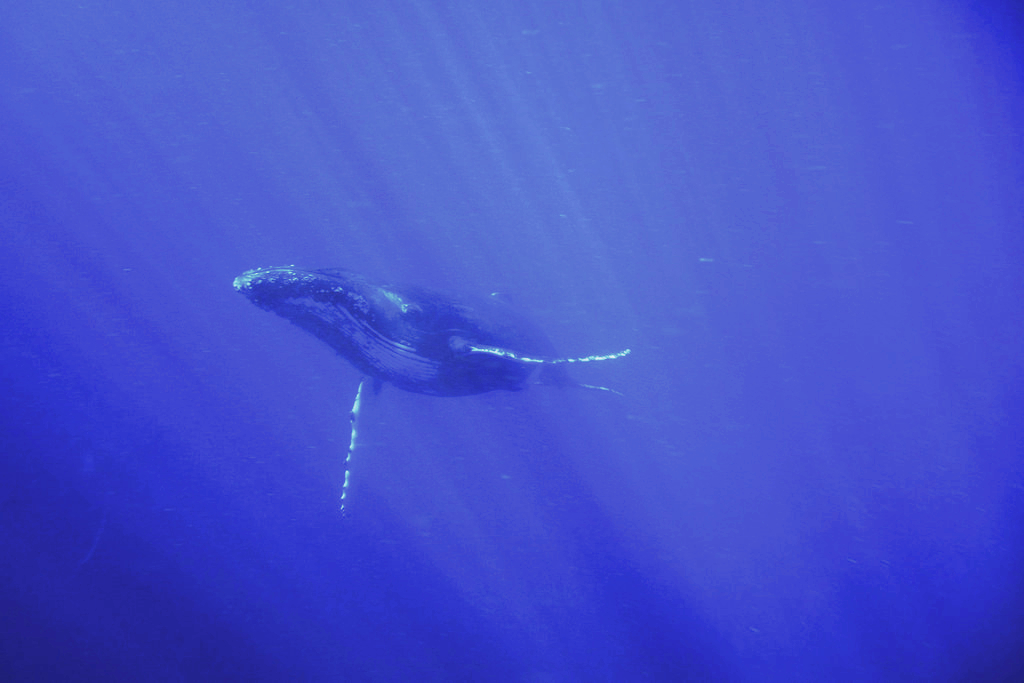
\includegraphics[width=5cm]{image/processed.jpg}
		}
		\quad
		\subfigure[image after sift]{
			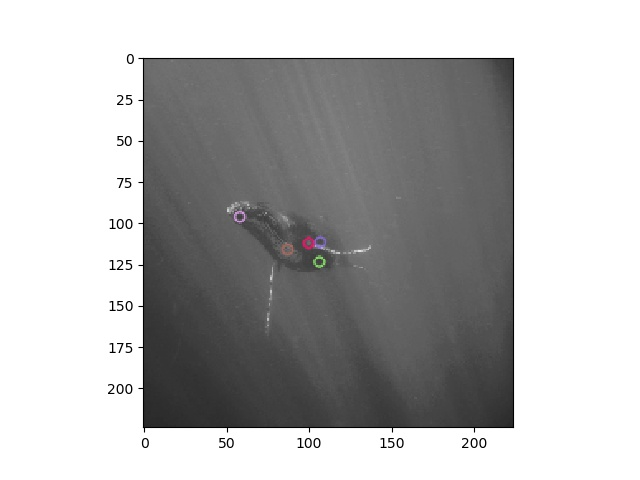
\includegraphics[width=5cm]{image/demo.jpg}
		}
		\caption{humpback}
		\label{Fig1}
	\end{figure}
\end{center}
\subsubsection{BOW}
\label{sec:z-score}
In this experiment, we used the BOW model to encode the descriptors extracted by sift, and set different clusters $k$ in $[8,16,32,64,128,256,512,1024]$. Besides, we normalized the feature vectors by z-score. After that, we fed encoded feature vectors into SVM for image classification and chose two different kernels of linear and rbf with the change of $C$.

\begin{table}[htbp]
	\centering
	\newcommand{\tabincell}[2]{\begin{tabular}{@{}#1@{}}#2\end{tabular}}
	\renewcommand\arraystretch{1.0}
	\caption{Accuracy of STFT features based on BOW(Z-Score) model}
	\label{base1}%
	\begin{tabular}{@{}p{1cm}<{\centering}|c|c|c|c}
		\hline
		\multirow{2}{*}{\diagbox[height=2\line,width=1.42cm,font=\tiny]{$k$}{Acc.}{$\mathit{M}$}} &
		\multicolumn{4}{c}{SIFT + BOW + SVM}\\
		\cline{2-5}
		& {C} & {linear kernel} & {C} & {rbf kernel}\\
		\hline
		8   & 0.0005 & 0.0699 & 0.5 & 0.1361\\
		8   & 0.001 & 0.0854 & 1.0 & 0.1394\\
		8   & 0.005 & 0.1138 & 5.0 & 0.1379\\
        8   & 0.01  & 0.1213 & 10 & 0.1369\\
        \hline
		16   & 0.0005  & 0.0882 & 0.5 & 0.1744\\
		16   & 0.001  & 0.1134 & 1.0 & 0.1786\\
		16   & 0.005  & 0.1470 & 5.0 & 0.1823\\
        16   & 0.01  & 0.1580 & 10 & 0.1763\\
        \hline
		32   & 0.0005  & 0.1183 & 0.5 & 0.1953\\
		32   & 0.001  & 0.1401 & 1.0 & 0.2018\\
		32   & 0.005  & 0.1767 & 5.0 & 0.1963\\
        32   & 0.01  & 0.1826 & 10 & 0.1885\\
        \hline
		64   & 0.0005  & 0.1495 & 0.5 & 0.2151\\
		64   & 0.001  & 0.1723 & 1.0 & 0.2205\\
		64   & 0.005  & 0.2049 & 5.0 & 0.2145\\
        64   & 0.01  & 0.2103 & 10 & 0.2059\\
        \hline
		128   & 0.0005  & 0.1774 & 0.5 & 0.2257\\
		128   & 0.001  & 0.2037 & 1.0 & 0.2342\\
		128   & 0.005  & 0.2210 & 5.0 & 0.2260\\
        128   & 0.01  & 0.2218 & 10 & 0.2211\\
        \hline
		256   & 0.0005  & 0.2054 & 0.5 & 0.2291\\
		256   & 0.001  & 0.2262 & 1.0 & 0.2434\\
		256   & 0.005  & 0.2321 & 5.0 & 0.2351\\
        256   & 0.01  & 0.2255 & 10 & 0.2317\\
        \hline
		512   & 0.0005  & 0.2293 & 0.5 & 0.2242\\
		512   & 0.001  & 0.2390 & 1.0 & 0.2444\\
		512   & 0.005  & 0.2272 & 5.0 & 0.2400\\
        512   & 0.01  & 0.2133 & 10 & 0.2359\\
        \hline
		1024   & 0.0005  & 0.2408 & 0.5 & 0.2231\\
		1024   & 0.001  & \textbf{0.2440} & 1.0 & 0.2511\\
		1024   & 0.005  & 0.2164 & 5.0 & \textbf{0.2488}\\
		1024   & 0.01  & 0.2036 & 10 & 0.2473\\
		\hline
	\end{tabular}
\end{table}

Our experiment results are shown in Tab. \ref{base1}. We can find that as k increases, the experimental results get better. We deem the reason is that when k is larger, the bag of words after codebook construction is larger, so the difference among the different types of images after feature encoding is also greater. Besides, we can find that rbf kernel performs better than linear kernel. We think this is because the dimension of the feature vector obtained by the BOW model is $k$, and rbf kernel is more suitable for classification with fewer feature dimensions than linear kernel. From the results we can see BOW's performance is poor because its highest accuracy is only $0.2488$. It is obvious because when mapping, BOW uses the  bag of words to quantify the image features for constructing a word frequency histogram. And the word frequency histogram is the encoded feature vector, so much information is lost.
\subsubsection{VLAD}
In this experiment, we used the VLAD model to encode the descriptors extracted by sift. The dimension of VLAD feature vector is $k*d$, where $k$ is the cluster number and $d$ is the dimension of each descriptor which equals 128. Because the feature dimension is too high, we use LDA and PCA for feature reduction. Besides, the experiments of VLAD consume time and computing resources, we can't set many different cluster numbers and large cluster numbers. So we only set $k$ in $[4,8,16]$ for experiments. After feature encoding and reduction, we fed encoded feature vectors into SVM for image classification and chose two different kernels of linear and rbf with the change of $C$.

\begin{table}[htbp]
	\centering
	\newcommand{\tabincell}[2]{\begin{tabular}{@{}#1@{}}#2\end{tabular}}
	\renewcommand\arraystretch{1.0}
	\caption{Accuracy of STFT features based on VLAD model after LDA}
	\label{base2}%
	\begin{tabular}{@{}p{1cm}<{\centering}|c|c|c|c}
		\hline
		\multirow{2}{*}{\diagbox[height=2\line,width=1.42cm,font=\tiny]{$k$}{Acc.}{$\mathit{M}$}} &
		\multicolumn{4}{c}{SIFT + VLAD + SVM + LDA}\\
		\cline{2-5}
		& {C} & {linear kernel} & {C} & {rbf kernel}\\
		\hline
		4   & 0.0005  & 0.2202 & 0.5 & 0.2722\\
		4   & 0.001  & 0.2524 & 1.0 & \textbf{0.2724}\\
		4   & 0.005  & 0.2669 & 5.0 & 0.2544\\
        4   & 0.01  & \textbf{0.2670} & 10 & 0.2493\\
        \hline
		8   & 0.0005 &0.2310 & 0.5 & 0.2645\\
		8   & 0.001 & 0.2506 & 1.0 & 0.2649\\
		8   & 0.005 & 0.2590 & 5.0 & 0.2519\\
        8   & 0.01  & 0.2578 & 10 & 0.2462\\
        \hline
		16   & 0.0005  & 0.2459 & 0.5 & 0.2517\\
		16   & 0.001  & 0.2542 & 1.0 & 0.2517\\
		16   & 0.005  & 0.2557 & 5.0 & 0.2451\\
		16   & 0.01  & 0.2540 & 10 & 0.2399\\
		\hline
	\end{tabular}
\end{table}

\begin{table}[htbp]
	\centering
	\newcommand{\tabincell}[2]{\begin{tabular}{@{}#1@{}}#2\end{tabular}}
	\renewcommand\arraystretch{1.0}
	\caption{Accuracy of STFT features based on VLAD model after PCA}
	\label{base3}%
	\begin{tabular}{@{}p{1cm}<{\centering}|c|c|c|c}
		\hline
		\multirow{2}{*}{\diagbox[height=2\line,width=1.42cm,font=\tiny]{$k$}{Acc.}{$\mathit{M}$}} &
		\multicolumn{4}{c}{SIFT + VLAD + SVM + PCA}\\
		\cline{2-5}
		& {C} & {linear kernel} & {C} & {rbf kernel}\\
		\hline
		4   & 0.0005  & 0.2389 & 0.5 & 0.0915\\
		4   & 0.001  & 0.2476 & 1.0 & 0.1574\\
		4   & 0.005  & 0.2513 & 5.0 & \textbf{0.1633}\\
        4   & 0.01  & 0.2513 & 10 & 0.1628\\
        \hline
		8   & 0.0005 & 0.2437 & 0.5 & 0.0590\\
		8   & 0.001 & 0.2499 & 1.0 & 0.0809\\
		8   & 0.005 & 0.2491 & 5.0 & 0.0886\\
        8   & 0.01  & 0.2489 & 10 & 0.0888\\
        \hline
		16   & 0.0005  & 0.2644 & 0.5 & 0.0509\\
		16   & 0.001  & \textbf{0.2660} & 1.0 & 0.0627\\
		16   & 0.005  & 0.2646 & 5.0 & 0.0683\\
		16   & 0.01  & 0.2625 & 10 & 0.0683\\
		\hline
	\end{tabular}
\end{table}

Our experiment results are shown in Tab. \ref{base2}, Tab. \ref{base3}. Generally speaking, it performs better when k is smaller. We deem the reason is that the larger the cluster number, the higher the feature dimension, and the more information is lost after dimensionality reduction. From the results we can find that linear kernel and rbf kernel perform similarly after LDA dimensionality reduction, but linear kernel performance is much better than rbf kernel after PCA dimensionality reduction. We think that the data put into the SVM is linearly separable, and the classification effect of the rbf kernel is greatly affected by the parameters. The parameters we choose are not suitable for data classification after VLAD feature encoding and PCA dimensionality reduction. Overall, VLAD performs better than BOW because it uses the residual of each descriptor with respect to its assigned cluster while BOW only involved simply counting the number of descriptors associated with each cluster in a codebook.
\subsubsection{Fisher Vector}
\label{sec:FV}
In this experiment, we used the FV model to encode the descriptors extracted by sift. The dimension of FV feature vector is $2*k*d$, where $k$ is the cluster number and $d$ is the dimension of each descriptor which equals 128. Because the feature dimension is too high, we use LDA and PCA for feature reduction like the VLAD experiment,. Besides, the experiments of FV also consume time and computing resources, we can't set many different cluster numbers and large cluster numbers. So we only set $k$ in $[4,8,16]$ for experiments. After feature encoding and reduction, we fed encoded feature vectors into SVM for image classification and chose two different kernels of linear and rbf with the change of $C$.

\begin{table}[htbp]
	\centering
	\newcommand{\tabincell}[2]{\begin{tabular}{@{}#1@{}}#2\end{tabular}}
	\renewcommand\arraystretch{1.0}
	\caption{Accuracy of STFT features based on FV model after LDA}
	\label{base4}%
	\begin{tabular}{@{}p{1cm}<{\centering}|c|c|c|c}
		\hline
		\multirow{2}{*}{\diagbox[height=2\line,width=1.42cm,font=\tiny]{$k$}{Acc.}{$\mathit{M}$}} &
		\multicolumn{4}{c}{SIFT + FV + SVM + LDA}\\
		\cline{2-5}
		& {C} & {linear kernel} & {C} & {rbf kernel}\\
		\hline
		4   & 0.0005  & 0.2504 & 0.5 & 0.2696\\
		4   & 0.001  & 0.2661 & 1.0 & \textbf{0.2703}\\
		4   & 0.005  & 0.2688 & 5.0 & 0.2589\\
        4   & 0.01  & \textbf{0.2689} & 10 & 0.2543\\
        \hline
		8   & 0.0005 & 0.2494 & 0.5 & 0.2578\\
		8   & 0.001 & 0.2594 & 1.0 & 0.2561\\
		8   & 0.005 & 0.2607 & 5.0 & 0.2468\\
        8   & 0.01  & 0.2560 & 10 & 0.2448\\
        \hline
		16   & 0.0005  & 0.2312 & 0.5 & 0.2334\\
		16   & 0.001  & 0.2351 & 1.0 & 0.2280\\
		16   & 0.005  & 0.2336 & 5.0 & 0.2198\\
		16   & 0.01  & 0.2315 & 10 & 0.2190\\
		\hline
	\end{tabular}
\end{table}

\begin{table}[htbp]
	\centering
	\newcommand{\tabincell}[2]{\begin{tabular}{@{}#1@{}}#2\end{tabular}}
	\renewcommand\arraystretch{1.0}
	\caption{Accuracy of STFT features based on FV model after PCA}
	\label{base5}%
	\begin{tabular}{@{}p{1cm}<{\centering}|c|c|c|c}
		\hline
		\multirow{2}{*}{\diagbox[height=2\line,width=1.42cm,font=\tiny]{$k$}{Acc.}{$\mathit{M}$}} &
		\multicolumn{4}{c}{SIFT + FV + SVM + PCA}\\
		\cline{2-5}
		& {C} & {linear kernel} & {C} & {rbf kernel}\\
		\hline
		4   & 0.0005  & 0.2420 & 0.5 & 0.0476\\
		4   & 0.001  & 0.2489 & 1.0 & 0.0829\\
		4   & 0.005  & 0.2530 & 5.0 & 0.0988\\
        4   & 0.01  & 0.2525 & 10 & \textbf{0.0988}\\
        \hline
		8   & 0.0005 & 0.2556 & 0.5 & 0.0445\\
		8   & 0.001 & 0.2606 & 1.0 & 0.0447\\
		8   & 0.005 & 0.2597 & 5.0 & 0.0453\\
        8   & 0.01  & 0.2587 & 10 & 0.0453\\
        \hline
		16   & 0.0005  & 0.2630 & 0.5 & 0.0436\\
		16   & 0.001  & 0.2655 & 1.0 & 0.0436\\
		16   & 0.005  & 0.2655 & 5.0 & 0.0436\\
		16   & 0.01  & \textbf{0.2658} & 10 & 0.0436\\
		\hline
	\end{tabular}
\end{table}

Our experiment results are shown in Tab. \ref{base4}, \ref{base5}. From the results we can find that FV performs better than BOW and VLAD. This is because Fisher Vector encodes a vector with richer image information which contains 1-order information and 2-order information. Besides in general, as k increases, the experimental results get worse. We deem the reason is that when k is larger, feature vectors resulting from feature encoding contain more redundant information. As for why when using PCA to reduce dimensionality, rbf kernel performs better than linear kernel, we think it is the same as the reason for this phenomenon in VLAD experiment.

\subsection{Selective Search + ResNet descriptors}

We used selective search to extract the local proposal of the images and use pretrained ResNet to extract the local descriptor, then used BOW, VLAD, FV to encode the features, and finally put them into the SVM for classification. As shown in Fig. \ref{kFig3}, when using selective search to extract image proposals in (a), we can limit the size of aim proposals and get the proposal-dropped one in (b), which can help us save the resources of computing.
\begin{center}
	\begin{figure}
		\centering
		\subfigure[original selective-search image]{
			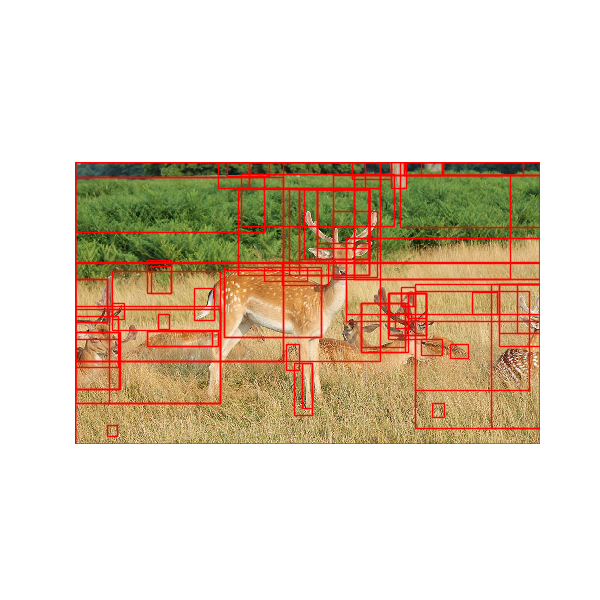
\includegraphics[width=5cm]{image/ssdemo.png}
		}
		\subfigure[proposal-dropped image]{
			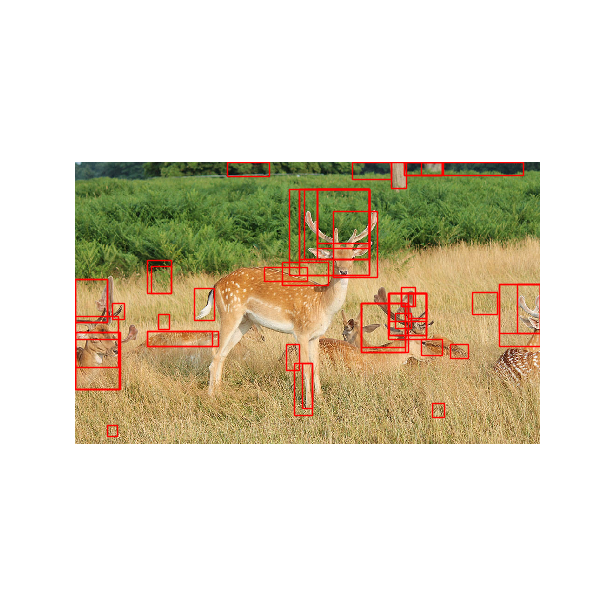
\includegraphics[width=5cm]{image/ssdemo_less.png}
		}
		\caption{ssdemo}
		\label{kFig3}
	\end{figure}
\end{center}
\subsubsection{BOW}
\label{sec:z-score}
In this experiment, we used the BOW model to encode the descriptors extracted by selective search + pretrained RseNet, and set different clusters $k$ in $[8,16,32,64,128,256,512,1024]$. Besides, we normalized the feature vectors by z-score. After that, we fed encoded feature vectors into SVM for image classification and chose two different kernels of linear and rbf with the change of $C$.

\begin{table}[htbp]
	\centering
	\newcommand{\tabincell}[2]{\begin{tabular}{@{}#1@{}}#2\end{tabular}}
	\renewcommand\arraystretch{1.0}
	\caption{Accuracy of Selective Search + pretrained RseNet features based on BOW(Z-Score) model}
	\label{kbase1}%
	\begin{tabular}{@{}p{1cm}<{\centering}|c|c|c|c}
		\hline
		\multirow{2}{*}{\diagbox[height=2\line,width=1.42cm,font=\tiny]{$k$}{Acc.}{$\mathit{M}$}} &
		\multicolumn{4}{c}{Selective Search + pretrained RseNet + BOW + SVM}\\
		\cline{2-5}
		& {C} & {linear kernel} & {C} & {rbf kernel}\\
		\hline
		8   & 0.001 & 0.0817 & 5 & 0.1080\\
        8   & 0.005  & 0.1032 & 10 & 0.1036\\
        \hline
		16   & 0.001  & 0.1105 & 5.0 & 0.1386\\
        16   & 0.005  & 0.1358 & 10 & 0.1299\\
        \hline
		32   & 0.001  & 0.1695 & 5.0 & 0.1847\\
        32   & 0.005  & 0.1984 & 10 & 0.1718\\
        \hline
		64   & 0.001  & 0.2108 & 5.0 & 0.2117\\
        64   & 0.005  & 0.2332 & 10 & 0.1977\\
        \hline
		128   & 0.001  & 0.2481 & 5.0 & 0.2424\\
        128   & 0.005  & 0.2629 & 10 & 0.2322\\
        \hline
		256   & 0.001  & 0.2626 & 5.0 & \textbf{0.2574}\\
        256   & 0.005  & 0.2734 & 10 & 0.2482\\
        \hline
		512   & 0.001  & 0.2586 & 5.0 & 0.2468\\
        512   & 0.005  & \textbf{0.2642} & 10 & 0.2393\\
        \hline
		1024   & 0.001  & 0.2548 & 5.0 & 0.2376\\
		1024   & 0.005  & 0.2561 & 10 & 0.2326\\
		\hline
	\end{tabular}
\end{table}

Our experiment results are shown in Tab. \ref{kbase1}. We can find that as k increases, the experimental results get better. We deem the reason is that when k is larger, the bag of words after codebook construction is larger, so the difference among the different types of images after feature encoding is also greater. From the results we can see BOW's performance is poor as its highest accuracy is only $0.2642$. It is obvious because when mapping, BOW uses the information of first level in codebook and information has been lost. Compared with SIFT method, we can find selective search + ResNet have poor performance, we deem the reason that We use pretrained ResNet rather than self-trained model.

\subsubsection{VLAD}
In this experiment, we used the VLAD model to encode the descriptors extracted by selective search + pretrained RseNet. The dimension of VLAD feature vector is $k*d$, where $k$ is the cluster number and $d$ is the dimension of each descriptor which equals 128. Because the feature dimension is too high, we use PCA for feature reduction. Besides, the experiments of VLAD consume time and computing resources, we can't set many different cluster numbers and large cluster numbers. So we only set $k$ in $[4,8]$ for experiments. After feature encoding and reduction, we fed encoded feature vectors into SVM for image classification and chose two different kernels of linear and rbf with the change of $C$.

\begin{table}[htbp]
	\centering
	\newcommand{\tabincell}[2]{\begin{tabular}{@{}#1@{}}#2\end{tabular}}
	\renewcommand\arraystretch{1.0}
	\caption{Accuracy of Selective Search + pretrained RseNet features based on VLAD model after PCA}
	\label{base3}%
	\begin{tabular}{@{}p{1cm}<{\centering}|c|c|c|c}
		\hline
		\multirow{2}{*}{\diagbox[height=2\line,width=1.42cm,font=\tiny]{$k$}{Acc.}{$\mathit{M}$}} &
		\multicolumn{4}{c}{Selective Search + pretrained RseNet + VLAD + SVM + PCA}\\
		\cline{2-5}
		& {C} & {linear kernel} & {C} & {rbf kernel}\\
		\hline
		4   & 0.001  & 0.4805 & 5.0 & 0.0719\\
        4   & 0.005  & \textbf{0.4864} & 10 & 0.0720\\
        \hline
		8   & 0.001 & 0.4281 & 5.0 & \textbf{0.1107}\\
        8   & 0.005  & 0.4412 & 10 & 0.1098\\
        \hline
	\end{tabular}
\end{table}

Our experiment results are shown in Tab. \ref{kbase2}. We conclude rbf ones performs better than linear one because rbf depends on initial parameters sampling while model is complecated. Overall, VLAD performs better than BOW because it uses the residual of each descriptor with respect to its assigned cluster while BOW only involved simply counting the number of descriptors associated with each cluster in a codebook. And we can find in VLAD, selective search + learning-based method have better performance than SIFT one because the former maintains more complete local information of images.
\subsubsection{Fisher Vector}
\label{sec:FV}
In this experiment, we used the FV model to encode the descriptors extracted by selective search + pretrained RseNet. The dimension of FV feature vector is $2*k*d$, where $k$ is the cluster number and $d$ is the dimension of each descriptor which equals 128. Because the feature dimension is too high, we use PCA for feature reduction like the VLAD experiment. Besides, the experiments of FV also consume time and computing resources, we can't set many different cluster numbers and large cluster numbers. So we only set $k$ in $[2,4]$ for experiments. After feature encoding and reduction, we fed encoded feature vectors into SVM for image classification and chose two different kernels of linear and rbf with the change of $C$.

\begin{table}[htbp]
	\centering
	\newcommand{\tabincell}[2]{\begin{tabular}{@{}#1@{}}#2\end{tabular}}
	\renewcommand\arraystretch{1.0}
	\caption{Accuracy of Selective Search + pretrained RseNet features based on FV model after PCA}
	\label{kbase5}%
	\begin{tabular}{@{}p{1cm}<{\centering}|c|c|c|c}
		\hline
		\multirow{2}{*}{\diagbox[height=2\line,width=1.42cm,font=\tiny]{$k$}{Acc.}{$\mathit{M}$}} &
		\multicolumn{4}{c}{Selective Search + pretrained RseNet + FV + SVM + PCA}\\
		\cline{2-5}
		& {C} & {linear kernel} & {C} & {rbf kernel}\\
		\hline
		2   & 0.001 & 0.3147 & 5.0 & 0.1548\\
        2   & 0.005  & 0.3440 & 10 & 0.1519\\
		\hline
		4   & 0.001  & 0.4637 & 5.0 & 0.0531\\
        4   & 0.005  & \textbf{0.4674} & 10 & 0.0531\\
		\hline
	\end{tabular}
\end{table}

Our experiment results are shown in Tab. \ref{kbase5}. From the results we can find that FV performs better than BOW but worse than VLAD. This is because Fisher Vector encodes 2-order information but our pretrained model can't extract the exact feature from local proposals. Besides in general, as k increases, the experimental results get worse. We deem the reason is that when k is larger, feature vectors resulting from feature encoding contain more redundant information. As for why when using PCA to reduce dimensionality, linear kernel performs better than rbf kernel, we think the reason that rbf performs poor if model is too complicated to get initial parameter sampling.

\section{Conclusion}
In this project, we extract local descriptors by two methods, SIFT and Selective Search + Resnet, and then encoding the descriptors by BOW, VLAD and FV, finally, we compare their performance in the SVM classification tasks. We can conclude Selective Search + Resnet method performance better although we use pretrained ResNet since our poor calculating resources. We deem the reason is that selective search maintains diversification information and avoid the noise of exhaustive search. Besides, we can find complicated model, such as 2-order FV and rbf ones, do not always perform well and it depends on the actual datasets and tasks.


\section{Futher discussion}
\subsubsection{Impact of scale method on BOW experiment}
We know that each dimension of the feature vector obtained by BOW is an integer. To avoid large dimensional differences, we need to standardize the feature vector. In section~\ref{sec:z-score}, we used Z-Score. In order to get the influence of standardized methods on the experimental results, in this experiment, we used the MaxMin.

\begin{table}[htbp]
	\centering
	\newcommand{\tabincell}[2]{\begin{tabular}{@{}#1@{}}#2\end{tabular}}
	\renewcommand\arraystretch{1.0}
	\caption{Accuracy of STFT features based on BOW(MaxMin-Scale) model}
	\label{base6}%
	\begin{tabular}{@{}p{1cm}<{\centering}|c|c|c|c}
		\hline
		\multirow{2}{*}{\diagbox[height=2\line,width=1.42cm,font=\tiny]{$k$}{Acc.}{$\mathit{M}$}} &
		\multicolumn{4}{c}{SIFT + BOW + SVM}\\
		\cline{2-5}
		& {C} & {linear kernel} & {C} & {rbf kernel}\\
		\hline
		8   & 0.0005 & 0.0430 & 0.5 & 0.0959\\
		8   & 0.001 & 0.0430 & 1.0 & 0.1080\\
		8   & 0.005 & 0.0430 & 5.0 & 0.1208\\
        8   & 0.01  & 0.0436 & 10 & 0.1247\\
        \hline
		16   & 0.0005  & 0.0435 & 0.5 & 0.0965\\
		16   & 0.001  & 0.0435 & 1.0 & 0.1136\\
		16   & 0.005  & 0.0435 & 5.0 & 0.1428\\
        16   & 0.01  & 0.0450 & 10 & 0.1556\\
        \hline
		32   & 0.0005  & 0.0456 & 0.5 & 0.0874\\
		32   & 0.001  & 0.0456 & 1.0 & 0.1154\\
		32   & 0.005  & 0.0464 & 5.0 & 0.1619\\
        32   & 0.01  & 0.0557 & 10 & 0.1773\\
        \hline
		64   & 0.0005  & 0.0440 & 0.5 & 0.0760\\
		64   & 0.001  & 0.0440 & 1.0 & 0.1063\\
		64   & 0.005  & 0.0486 & 5.0 & 0.1711\\
        64   & 0.01  & 0.0608 & 10 & 0.1870\\
        \hline
		128   & 0.0005  & 0.0442 & 0.5 & 0.0636\\
		128   & 0.001  & 0.0442 & 1.0 & 0.0977\\
		128   & 0.005  & 0.0556 & 5.0 & 0.1708\\
        128   & 0.01  & 0.0743 & 10 & 0.1904\\
        \hline
		256   & 0.0005  & 0.0433 & 0.5 & 0.0587\\
		256   & 0.001  & 0.0433 & 1.0 & 0.0826\\
		256   & 0.005  & 0.0657 & 5.0 & 0.1730\\
        256   & 0.01  & 0.0975 & 10 & 0.2006\\
        \hline
		512   & 0.0005  & 0.0468 & 0.5 & 0.0523\\
		512   & 0.001  & 0.0468 & 1.0 & 0.0756\\
		512   & 0.005  & 0.0916 & 5.0 & 0.1738\\
        512   & 0.01  & 0.1345 & 10 & \textbf{0.2071}\\
        \hline
		1024   & 0.0005  & 0.0430 & 0.5 & 0.0439\\
		1024   & 0.001  & 0.0442 & 1.0 & 0.0568\\
		1024   & 0.005  & 0.0568 & 5.0 & 0.1399\\
		1024   & 0.01  & \textbf{0.1418} & 10 & 0.1772\\
		\hline
	\end{tabular}
\end{table}

Our experiment results are shown in Tab. \ref{base6}. We can find that Z-Score performs better than MaxMin.
We speculate that there may be outliers in the feature vector that affect the experimental results. Therefore Z-Score is more suitable for this project.
\subsubsection{FV containing only first-order information}
We know that FV uses gradient vectors of likelihood functions to encode pictures. In general, it contains both first-order information (expectation) and second-order information (variance). Therefore, in this section, we set the FV to include only first-order information, and conduct a comparative experiment with section~\ref{sec:FV}.

\begin{table}[htbp]
	\centering
	\newcommand{\tabincell}[2]{\begin{tabular}{@{}#1@{}}#2\end{tabular}}
	\renewcommand\arraystretch{1.0}
	\caption{Accuracy of STFT features based on FV(1-order) model after LDA}
	\label{base7}%
	\begin{tabular}{@{}p{1cm}<{\centering}|c|c|c|c}
		\hline
		\multirow{2}{*}{\diagbox[height=2\line,width=1.42cm,font=\tiny]{$k$}{Acc.}{$\mathit{M}$}} &
		\multicolumn{4}{c}{SIFT + FV + SVM + LDA}\\
		\cline{2-5}
		& {C} & {linear kernel} & {C} & {rbf kernel}\\
		\hline
		4   & 0.0005  & 0.2405 & 0.5 & 0.2698\\
		4   & 0.001  & 0.2626 & 1.0 & \textbf{0.2723}\\
		4   & 0.005  & \textbf{0.2702} & 5.0 & 0.2576\\
        4   & 0.01  & 0.2678 & 10 & 0.2494\\
        \hline
		8   & 0.0005 & 0.2446 & 0.5 & 0.2694\\
		8   & 0.001 & 0.2610 & 1.0 & 0.2662\\
		8   & 0.005 & 0.2686 & 5.0 & 0.2552\\
        8   & 0.01  & 0.2653 & 10 & 0.2493\\
        \hline
		16   & 0.0005  & 0.2487 & 0.5 & 0.2555\\
		16   & 0.001  & 0.2561 & 1.0 & 0.2538\\
		16   & 0.005  & 0.2550 & 5.0 & 0.2471\\
		16   & 0.01  & 0.2515 & 10 & 0.2428\\
		\hline
	\end{tabular}
\end{table}

\begin{table}[htbp]
	\centering
	\newcommand{\tabincell}[2]{\begin{tabular}{@{}#1@{}}#2\end{tabular}}
	\renewcommand\arraystretch{1.0}
	\caption{Accuracy of STFT features based on FV model after PCA}
	\label{base8}%
	\begin{tabular}{@{}p{1cm}<{\centering}|c|c|c|c}
		\hline
		\multirow{2}{*}{\diagbox[height=2\line,width=1.42cm,font=\tiny]{$k$}{Acc.}{$\mathit{M}$}} &
		\multicolumn{4}{c}{SIFT + FV + SVM + PCA}\\
		\cline{2-5}
		& {C} & {linear kernel} & {C} & {rbf kernel}\\
		\hline
		4   & 0.0005  & 0.2440 & 0.5 & 0.1214\\
		4   & 0.001  & 0.2496 & 1.0 & 0.1659\\
		4   & 0.005  & 0.2507 & 5.0 & 0.1733\\
        4   & 0.01  & 0.2473 & 10 & \textbf{0.1733}\\
        \hline
		8   & 0.0005 & 0.2496 & 0.5 & 0.0588\\
		8   & 0.001 & 0.2560 & 1.0 & 0.1022\\
		8   & 0.005 & 0.2568 & 5.0 & 0.1154\\
        8   & 0.01  & 0.2558 & 10 & 0.1154\\
        \hline
		16   & 0.0005  & 0.2593 & 0.5 & 0.0445\\
		16   & 0.001  & \textbf{0.2615} & 1.0 & 0.0599\\
		16   & 0.005  & 0.2613 & 5.0 & 0.0702\\
		16   & 0.01  & 0.2604 & 10 & 0.0702\\
		\hline
	\end{tabular}
\end{table}

Our experiment results are shown in Tab. \ref{base7}, \ref{base8}. From the results we can find that FV containing only first-order information even performs slightly better than FV containing first- and second-order information. From this we can deduce that sometimes FV can only use first-order information for feature encoding, which also reduces the requirements for computing resources. Besides, we can find that also containing only first-order information, FV performs better than VLAD. We think the reason is that GMM clustering can extract feature information better than K-Means clustering.

\bibliography{Prj3}
\end{document}